%======================================================================
\section{Verification with the Voting-Machine Files (N1, N2, N4, N5)}
\label{sec:machine}

Statistical tests can only say whether the published counts look like
honest counts. The files that each voting machine writes at the end of the
day allow a direct check: whether the published result is what the machine
recorded, and whether the files were altered afterwards. The TSE published
these files for every section of both rounds \cite{tse2026urna}. We
processed 499,207 sections per round, which covers every official section
plus one or two sections abroad with files but no votes.

\subsection{Recount of the digital vote record (N1)}

The RDV stores each vote as cast, office by office, in random order. We
decoded every RDV, recounted its votes and compared them with the BU of the
same section, office by office; then we compared the BU of each section with
the official per-section CSV used in Sections~\ref{sec:results} and
\ref{sec:cross}. Table~\ref{tab:n1} summarizes the result. The recount
matched the BU in all 3,030,617 section--office comparisons of the two
rounds: 2,490,800 in the first round (President, Senator, Governor and
federal, state and district deputies, plus 10 comparisons of another
contest held on the same day) and 539,817 in the runoff (President,
Governor in the states with a gubernatorial runoff and 871 comparisons of
municipal or supplementary contests). One section in Maranh\~ao had no RDV
file in the first round and could not be recounted. In 31 sections in the
first round and 29 in the runoff the BU had been generated by the counting
system rather than by the machine (29 sections abroad in each round and 2
in Minas Gerais in the first round); their RDVs also matched. The BUs, in
turn, reproduced the official per-section results without a single vote of
difference in any section, so the national totals are identical
(Table~\ref{tab:n1tot}).

\begin{table}[ht]
\caption{Recount of the RDV against the BU (N1)}
\label{tab:n1}
\centering\scriptsize
\begin{tabular}{@{}l r r@{}}
\toprule
 & \textbf{1st round} & \textbf{Runoff} \\
\midrule
Official sections & 499,206 & 499,205 \\
Sections with machine files & 499,207 & 499,207 \\
BU from the machine / from counting system & 499,176 / 31 & 499,178 / 29 \\
Sections without RDV & 1 & 0 \\
Section--office comparisons & 2,490,800 & 539,817 \\
\quad of which divergent & 0 & 0 \\
Sections with BU $\neq$ official CSV & 0 & 0 \\
\bottomrule
\end{tabular}
\end{table}

\begin{table}[ht]
\caption{National totals: BU files and official result (President)}
\label{tab:n1tot}
\centering\scriptsize
\begin{tabular}{@{}l l r r@{}}
\toprule
\textbf{Round} & \textbf{Option} & \textbf{BU files} & \textbf{Difference} \\
\midrule
1st & F.\ Bolsonaro (22) & 56,104,503 & 0 \\
1st & Lula (13) & 53,879,538 & 0 \\
1st & Others (11 candidates) & 9,321,993 & 0 \\
1st & Blank / null & 2,300,798 / 3,669,003 & 0 \\
2nd & Lula (13) & 64,256,232 & 0 \\
2nd & F.\ Bolsonaro (22) & 59,826,041 & 0 \\
2nd & Blank / null & 1,430,496 / 2,723,305 & 0 \\
\bottomrule
\end{tabular}
\end{table}

\subsection{Integrity and signatures (N2)}

Each machine signs a file (\texttt{.vsc}) that contains the SHA-512
\cite{fips180} of the BU, the RDV and the log, with a key unique to the
machine and its certificate embedded. We recomputed the three hashes of every
section and verified the hardware signature: ECDSA over the P-521 curve with
SHA-512 \cite{fips186} for models UE2013 and UE2015, and Ed521 (EdDSA over
the E-521 Edwards curve \cite{aranha2013,fips186}) for models UE2020 and
UE2022, the scheme the TSE reports for its newer machines \cite{tse2023tps}.
All 998,414 signatures were valid and no hash differed from the signed value
(Table~\ref{tab:n2}); the only hashes not compared were those of the missing
RDV above and of one missing log. Two limits apply. The chain from each
machine certificate to the TSE root authority was not verified, because the
root certificates are not published; and the second, software signature,
which uses a non-public algorithm, was not verified either. The test
therefore shows that the files were not altered after being signed by the
key whose certificate they carry, not that this key belongs to a genuine
machine.

\begin{table}[ht]
\caption{Hashes and hardware signatures by machine model (N2)}
\label{tab:n2}
\centering\scriptsize
\begin{tabular}{@{}l l r r r@{}}
\toprule
\textbf{Model} & \textbf{Signature} & \textbf{1st round} & \textbf{Runoff} & \textbf{Failures} \\
\midrule
UE2013 & ECDSA P-521 & 11,921 & 12,455 & 0 \\
UE2015 & ECDSA P-521 & 88,064 & 87,502 & 0 \\
UE2020 & Ed521 & 200,463 & 200,504 & 0 \\
UE2022 & Ed521 & 198,759 & 198,746 & 0 \\
\midrule
Total & & 499,207 & 499,207 & 0 \\
\bottomrule
\end{tabular}
\end{table}

\subsection{Voting rhythm in the logs (N4)}

The log records each event of the machine with a timestamp, including every
vote cast. In the 499,176 (first round) and 499,177 (runoff) sections with a
machine log, no vote was recorded before the machine was declared ready or
after the session was closed; the largest number of votes in any single
minute was 3 in the first round and 4 in the runoff, and no section had two
votes less than 5~seconds apart. These are the marks that a burst of
inserted votes would leave, and none appeared.

Figure~\ref{fig:n4} shows the share of votes per hour. In the runoff, voting
was concentrated in the morning and practically ended at 17:00 (0.03\% of
the votes after that time); in the first round, 2.97\% of the votes were
cast after 17:00, by voters already in line. A likely reason is that the
first round asked for six offices and the runoff for one or two, so each
voter took longer and queues were longer at closing time. Within
municipalities, sections with a larger share of late votes gave slightly
more votes to Lula in the first round (+0.009 in the logit per percentage
point of late votes; $z=11.5$) but not in the runoff ($p=0.13$). These late
votes are in the RDV and were recounted in N1, so the association describes
where queues formed, not an anomaly in the count. In 153 sections per round
votes were time-stamped before 08:00 local time, but always after the
machine was ready, which points to clock offsets rather than early voting.
In 16 section--rounds (9 and 7) the number of vote events in the log
differed from the BU; the 7 runoff cases also contained events from
another date (for example, a log with 612 vote events against 308 votes in
the BU in a section of Esp\'irito Santo); in all of them the RDV recount
matched the BU and the signatures were valid. They are listed for manual
inspection.

\begin{figure}[ht]
\centering
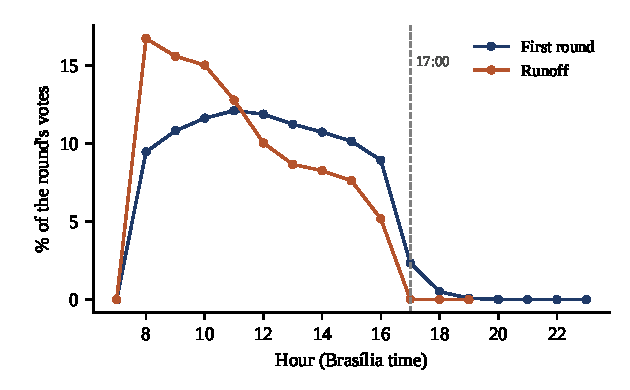
\includegraphics[width=\linewidth]{Figures/fig_n4_hourly.pdf}
\caption{Share of the votes of each round cast per hour (Bras\'ilia time),
from the logs of all voting machines.}
\label{fig:n4}
\end{figure}

\subsection{Releases without biometrics (N5)}

The BU reports how many voters were enabled by fingerprint and how many by
biographic data (birth year) when the fingerprint was not recognized. The
median share of biographic releases per section was 6.1\% in both rounds
(99th percentile: 19\%). Using a robust $z$ within the municipality, 589
sections in the first round and 517 in the runoff had an unusually high
share ($z>6$; 0.1\% of sections). The one with the highest $z$, in Minas
Gerais, enabled 266 of its 290 voters by biographic data, and in others the
share reached 99\%, which suggests a failing
fingerprint reader and should be checked in the section's minutes. The
share of biographic releases and Lula's vote are associated: in the top
decile of biographic releases Lula received 0.59 percentage points more than
the municipal mean in the first round and 0.28 in the runoff. After
controlling for the share of voters with registered biometrics and for the
municipality, the coefficient was small and significant only in the first
round (+0.0033 in the logit per point; $p=0.03$; runoff $p=0.32$).
Fingerprint recognition is known to fail more often for older voters and
manual workers, groups that leaned toward Lula (Section~\ref{sec:extended});
this hypothesis was not tested directly.

%======================================================================
\section{Further Statistical Tests (N6--N12)}
\label{sec:extended}

Table~\ref{tab:nsummary} summarizes the seven further statistical tests.
Unless stated otherwise, they use the runoff and the share of Lula among the
two finalists; N7 and N8 use sections with at least 50 votes, N9 and N12
sections with at least 20, N12 only municipalities with at least 20
sections, and N11 sections with at least 50 eligible voters.

\begin{table*}[ht]
\caption{Further statistical tests: method and main result}
\label{tab:nsummary}
\centering\scriptsize
\begin{tabular}{@{}l L{3.3cm} L{5.4cm} L{6.4cm}@{}}
\toprule
\textbf{\#} & \textbf{Test} & \textbf{Method} & \textbf{Main result} \\
\midrule
N6 & Machine model & Regression with polling-place fixed effect, SE clustered by municipality, BH & No model effect on vote, turnout or blank/null within the same polling place (all $q\geq0.29$) \\
N7 & Electorate profile & Logit with municipality fixed effect, beta-binomial over-dispersion \cite{williams1982}, predictive checks \cite{gelman1996} & Expected signs; 1,024 sections flagged (0.21\%); model under-predicts very high Lula shares \\
N8 & Panel 2022$\to$2026 & Change of logit share in the same section, centred on municipality, robust $z$ & $r=0.973$; 822 sections with $|z|>6$ (0.19\%), 585 of them away from the winner \\
N9 & Round-number spikes & Resampled kernel idea \cite{rozenas2017}: binomial resampling, 500 replicates, multiples of 5\% & Only Lula, first round: +247 sections (0.05\%; $p=0.008$), spread over 30--50\% \\
N10 & Spatial clustering & Local Moran \cite{anselin1995}, 8 nearest polling places, permutations, BH & No significant cluster of extreme residuals; test under-powered (see text) \\
N11 & Machine learning & Random forest \cite{breiman2001,wright2017} trained on 300,000 synthetic sections & 2 real sections flagged vs.\ 499 expected at 0.1\% false-positive rate \\
N12 & Local multimodality & Dip test \cite{hartigan1985} per municipality, BH; 2022 as control & 8 of 3,932 municipalities in 2026 vs.\ 4 of 3,774 in 2022; all contain indigenous lands \\
\bottomrule
\end{tabular}
\end{table*}

\paragraph{Machine model (N6)} Without controls, sections with the oldest
model (UE2013) gave Lula a larger share (51.2\% of the two finalists in the
first round, against 48.7--49.2\% for the other models) and had lower
turnout (71.6\% against 78.5--79.4\%). These are differences of place: older
machines are used in particular regions. Within the same polling place ---
7,896 places in the first round and 8,525 in the runoff had machines of two
or more models --- no model had a significant effect on Lula's share, turnout
or blank and null votes (all BH $q\geq0.29$; largest coefficient 0.037 in the
logit). The model reported in the machine signature agreed with the model in
the TSE detail file in all but 6 sections.

\paragraph{Electorate profile (N7)} A logit model with municipality fixed
effects relates each section's vote to the profile of its voters
\cite{tse2026eleitorado}. The coefficients have the expected signs: Lula's share grows
with the shares of women, voters aged 16--24, voters with low schooling and
voters with registered biometrics, and falls with the shares aged 45--59 and
60 or more; the profile explains 26\% of the within-municipality variance of
the runoff. Over-dispersion is small ($\rho=0.013$). Using BH ($q<0.001$),
1,024 runoff sections (0.21\%) deviate from the model, about 190 of them
in indigenous villages according to the polling-place name. Predictive
simulation reproduces the within-municipality dispersion of Lula's
first-round share ($p=0.52$), slightly over-predicts it in the runoff
(standard deviation 0.0734 observed against 0.0746 simulated) and misses the
tails: there are 6,714 runoff sections with more than 90\% for Lula against
4,734 simulated. The profile, which is available only by broad categories, does
not capture homogeneous communities, the same limitation seen in T1.

\paragraph{Panel 2022--2026 (N8)} 443,458 runoff sections kept the same
number and polling place as in 2022 and had at least 50 votes for the two
finalists in both years. Lula's share in 2026 is strongly correlated with
his share in 2022 ($r=0.973$; Figure~\ref{fig:n8}), with a mean change of
+0.29 percentage points and state means between $-3.0$ (TO) and $+4.3$
(DF). With a robust $z$ centred on the municipality, 822 sections (0.19\%)
changed more than six robust deviations; 585 moved \emph{away} from Lula
and 237 toward him. About 90 are in indigenous villages; the most extreme is in
the Maxakali indigenous land in Minas Gerais, where Lula fell from 99.5\% to
70.1\%. The opponent in 2026 was a different candidate from 2022, so local
swings are expected. Indigenous sections are over-represented among the
extreme swings, as remote areas were in Turkey \cite{klimek2023}, but here
the swings mostly ran against the winner.

\begin{figure}[ht]
\centering
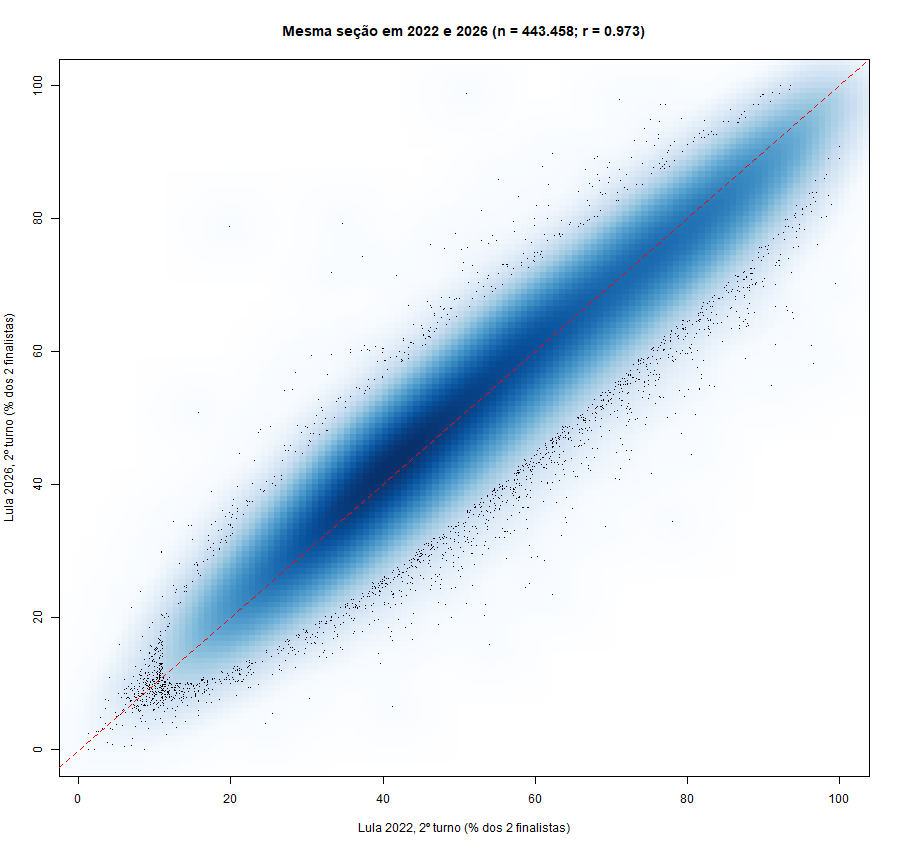
\includegraphics[width=0.85\linewidth]{Figures/N8_painel_2022_2026.png}
\caption{Same section in 2022 and 2026: Lula's share of the two finalists in
the 2022 runoff (x axis) and in the 2026 runoff (y axis); $n=443{,}458$;
dashed line: no change. The dots are the sections in the least dense
regions.}
\label{fig:n8}
\end{figure}

\paragraph{Round-number spikes (N9)} For each section we counted whether
the share fell within 0.05 percentage points of a multiple of 5\%, and
compared the total with 500 binomial resamples of the same sections, which
keep the spikes that small denominators create naturally. There was no
excess for Fl\'avio Bolsonaro in either round, for Lula in the runoff, or
for turnout. For Lula in the first round there were 247 more sections at
round values than expected (0.05\% of sections; 95\% interval 0.01--0.09\%;
$p=0.008$), spread over the foci between 30\% and 50\% rather than
concentrated on high round values such as those found in falsified Russian
results \cite{kobak2016}. Given the number of series tested (six), this
single small excess is weak evidence.

\paragraph{Spatial clustering (N10)} Polling places were geocoded and
linked to their eight nearest neighbours within the state. Global Moran's
$I$ was low for the residuals of the cross-round test (median across states
0.025) and of the panel (0.039), and higher for the profile model (0.200),
which indicates spatially structured variables missing from that model. No
local cluster of extreme residuals reached significance. This null result
is not informative, however: with 199 permutations the smallest attainable
$p$-value is 0.005, which cannot survive the BH correction over about 90,000
polling places. The test must be rerun with many more permutations or with
analytical inference before it can be interpreted.

\paragraph{Machine learning (N11)} Following Zhang, Alvarez and Levin
\cite{zhang2019}, we generated 150,000 clean synthetic sections, from the real
first round of each section plus a typical change between rounds, and
150,000 manipulated ones, with ballot stuffing, vote swapping or fabricated
round numbers, and trained a random forest of 300 trees on 11 features. On
held-out synthetic data the area under the ROC curve was 0.863 (0.858 for
stuffing, 0.794 for swapping and 0.938 for fabrication). With the threshold
set for a false-positive rate of 0.1\% on clean synthetic sections, the
model would flag about 499 of the 498,950 real sections if they were all
clean; it flagged 2, both in the same S\~ao Paulo polling place that
appeared in T6 and T8. At this threshold, however, sensitivity is low
(18\% for stuffing, 15\% for swapping and 0.3\% for fabrication), so the
test is a conservative screen. The distribution of predicted probabilities
for real sections is bimodal, with a secondary mode near 0.75 holding
roughly a tenth of the sections (Figure~\ref{fig:n11}). The last digit of Lula's
count is the second most important feature, and fabricated counts in the
training data end in zero; since about 10\% of honest counts end in zero
(T2), this mode is probably an artifact of that feature, which should be
confirmed by refitting the model without it.

\begin{figure}[ht]
\centering
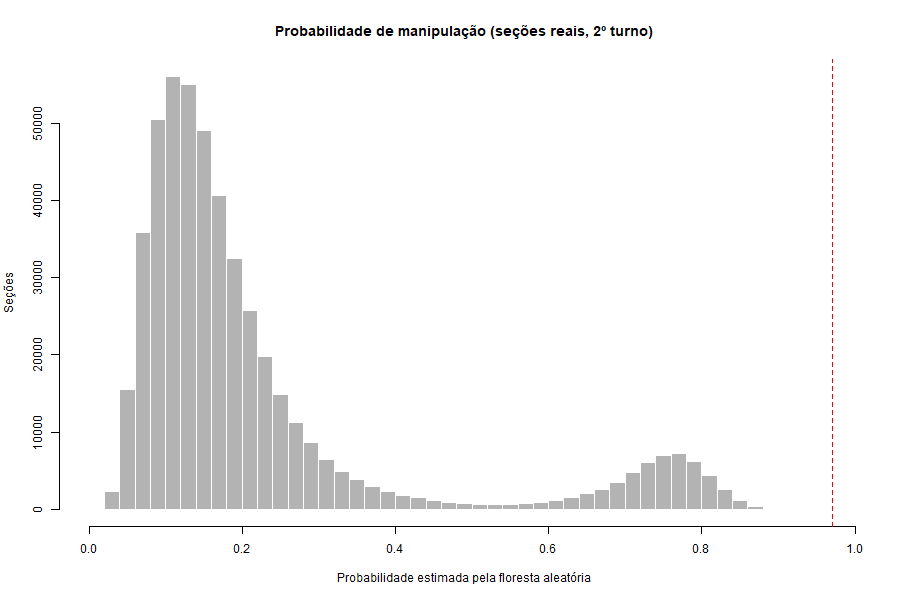
\includegraphics[width=\linewidth]{Figures/N11_ml_probabilidades.png}
\caption{Probability of manipulation estimated by the random forest for the
real runoff sections (x axis) and number of sections (y axis); dashed line:
threshold for a 0.1\% false-positive rate.}
\label{fig:n11}
\end{figure}

\paragraph{Local multimodality (N12)} A mixture of two voting regimes inside
a municipality --- for example, a group of inflated sections --- produces a
bimodal distribution of the vote share. Of the 3,932 municipalities with at
least 20 sections in the 2026 runoff, 8 had a significant dip test (BH
$q<0.05$), against 4 of 3,774 in the 2022 runoff. Four are the same in both
years (S\~ao Paulo de Oliven\c{c}a, S\~ao Gabriel da Cachoeira and Tabatinga,
in Amazonas, and Japor\~a, in Mato Grosso do Sul); the other four are
Campin\'apolis (MT), Tocant\'inia (TO), Ipua\c{c}u (SC) and Amambai (MS),
which were not multimodal, or had too few sections to be tested, in 2022.
All eight contain indigenous lands, where sections in villages vote very
differently from urban sections.

\subsection{Remaining checks}

Three checks remain open. N3, the comparison of the tally sheets printed and
posted at the sections with the published files, requires a stratified
random sample of the QR codes collected by observers. The certificate chain
of the machine signatures can only be verified if the TSE publishes the root
certificates. And the classification of flagged sections by type of polling
place should use the official register instead of keywords.


